\section{Results}
\label{sec:results}

\subsection{Descriptive Statistics}

Table~\ref{tab:descriptive} reports summary statistics for the key variables.

\begin{table}[H]
\centering
\caption[Descriptive Statistics]{Descriptive Statistics (August 2020 -- January 2026)}
\label{tab:descriptive}
\begin{tabular}{@{}lrrrr@{}}
\toprule
\textbf{Variable} & \textbf{Mean} & \textbf{Std Dev} & \textbf{Min} & \textbf{Max} \\
\midrule
BTC Price (\$) & 51,647 & 30,235 & 10,132 & 124,753 \\
MSTR Price (\$) & 116.55 & 121.29 & 13.49 & 473.83 \\
NAV Premium (\%) & 196.0 & 230.3 & $-$40.6 & 1,501.6 \\
BTC 30d Vol (\%) & 45.58 & 16.48 & 14.11 & 98.91 \\
MSTR 30d Vol (\%) & 88.38 & 31.23 & 35.95 & 183.97 \\
\bottomrule
\end{tabular}
\end{table}

The average NAV premium of 196\% reflects the fact that MSTR has traded at a persistent premium to its Bitcoin holdings throughout most of the sample period. The premium exhibits enormous volatility (standard deviation of 230 percentage points), ranging from $-41\%$ to over 1,500\%. The extreme upper values reflect the early period (2020--2021) when BTC holdings were small relative to the legacy software business valuation. The median premium of 131\% is more representative of typical conditions.

\subsection{Stress Testing the Capital Structure}

\subsubsection{Sensitivity to BTC Price}

Table~\ref{tab:sensitivity} shows how Strategy's capital structure metrics change with BTC price.

\begin{table}[H]
\centering
\caption{Capital Structure Sensitivity to BTC Price}
\label{tab:sensitivity}
\begin{tabular}{@{}lccc@{}}
\toprule
\textbf{BTC Price} & \textbf{NAV} & \textbf{Asset/Debt} & \textbf{Equity Value} \\
\midrule
\$120,000 (+26\%) & \$85.6B & 5.37$\times$ & \$69.7B \\
\$95,000 (Base) & \$67.8B & 4.25$\times$ & \$51.8B \\
\$75,000 ($-$21\%) & \$53.5B & 3.36$\times$ & \$37.6B \\
\$55,000 ($-$42\%) & \$39.2B & 2.46$\times$ & \$23.3B \\
\$35,000 ($-$63\%) & \$25.0B & 1.57$\times$ & \$9.0B \\
\$22,346 ($-$76\%) & \$15.9B & 1.00$\times$ & \$0 \\
\bottomrule
\end{tabular}
\end{table}

The key insight is leverage. A 50\% BTC decline doesn't produce a 50\% equity decline; it produces a 65\% decline (from \$51.8B to \$17.9B at \$47,500 BTC). As BTC falls, equity absorbs losses first, amplifying percentage moves in both directions. At \$35,000 BTC, equity has fallen 83\% while BTC is down 63\%. At \$22,346, equity is worthless.

Strategy's current position provides substantial cushion. The 4.25$\times$ asset/debt ratio means Bitcoin would need to fall 76\% before equity faces complete wipeout. This is healthier than earlier in the company's history, when smaller BTC holdings meant tighter breakevens.

\subsubsection{Breakeven Analysis}

Table~\ref{tab:breakeven} reports the BTC price at which each capital layer faces impairment.

\begin{table}[H]
\centering
\caption{Breakeven BTC Prices by Capital Layer}
\label{tab:breakeven}
\begin{tabular}{@{}lrr@{}}
\toprule
\textbf{Capital Layer} & \textbf{Claim Amount} & \textbf{Breakeven BTC} \\
\midrule
Convertible Debt & \$7.41B & \$10,391 \\
STRF (Senior Preferred) & \$1.37B & \$12,311 \\
STRC (Variable Preferred) & \$3.38B & \$17,048 \\
STRE (Euro Preferred) & \$0.80B & \$18,170 \\
STRK (Convert Preferred) & \$1.54B & \$20,328 \\
STRD (Junior Preferred) & \$1.44B & \$22,346 \\
Common Equity & -- & \$22,346 \\
\bottomrule
\end{tabular}
\end{table}

Common equity gets wiped out at approximately \$22,346 BTC (a 76\% decline). Senior convertible debt doesn't face impairment until \$10,391 (an 89\% decline). The capital structure provides meaningful cushion for senior claims.

\subsubsection{Critical Thresholds}

Three thresholds matter for understanding how the strategy unravels:

\textbf{Threshold 1: Capital Market Access} ($\sim$\$35,000 BTC). At this level, equity has declined 83\% and the asset/debt ratio compresses to 1.57$\times$. Strategy likely loses the ability to issue ATM equity at attractive terms. The reflexive loop weakens.

\textbf{Threshold 2: Preferred Dividend Strain} ($\sim$\$28,000 BTC). NAV falls to approximately \$20.0 billion against \$15.9 billion in claims. The \textasciitilde\$890M annual servicing burden represents roughly 22\% of remaining equity value. The USD reserve becomes critical.

\textbf{Threshold 3: Equity Wipeout} ($\sim$\$22,350 BTC). Asset value equals total claims. Common equity is worthless. Preferred dividends are at risk.

\subsection{NAV Premium Persistence}

Table~\ref{tab:regression} reports the autoregressive results.

\begin{table}[H]
\centering
\caption{NAV Premium Persistence}
\label{tab:regression}
\begin{tabular}{@{}lc@{}}
\toprule
\textbf{Variable} & \textbf{Coefficient} \\
\midrule
$Premium_{t-1}$ & 1.002*** \\
& (0.006) \\
Constant & $-$0.003 \\
& (0.009) \\
\midrule
Observations & 1,059 \\
$R^2$ & 0.994 \\
\bottomrule
\multicolumn{2}{l}{\footnotesize *** p<0.01}
\end{tabular}
\end{table}

The lagged premium coefficient of 1.002 with an $R^2$ of 0.994 tells a simple story: premium states are sticky. Once MSTR trades at a premium (or discount), it tends to stay there. The coefficient near unity indicates a near-unit-root process --- the premium drifts in prolonged regimes rather than mean-reverting. This persistence is what allows Strategy to exploit premium windows for extended capital raising campaigns rather than racing to issue before the window closes.

\subsection{Event Study: Capital Raises and Premium Windows}

Table~\ref{tab:event_study} reports average NAV premiums in the windows around capital raise announcements.

\begin{table}[H]
\centering
\caption{NAV Premium Around Capital Raise Events}
\label{tab:event_study}
\begin{tabular}{@{}lc@{}}
\toprule
\textbf{Window} & \textbf{Average NAV Premium} \\
\midrule
20 days pre-event & 134.3\% \\
10 days pre-event & 129.3\% \\
5 days pre-event & 127.4\% \\
5 days post-event & 125.3\% \\
10 days post-event & 121.9\% \\
\bottomrule
\multicolumn{2}{l}{\footnotesize N = 23 capital raise events (Oct 2024 -- Nov 2025).}
\end{tabular}
\end{table}

Strategy raises capital at substantial premiums to NAV. In the 5 trading days before announcements, the stock trades at an average 127\% premium --- roughly 2.3$\times$ NAV. Premiums decline in the days following issuance, falling to 122\% at 10 days post-event, consistent with the market pricing in dilution from new share issuance.

Figure~\ref{fig:event_study} visualizes the pattern.

\begin{figure}[H]
    \centering
    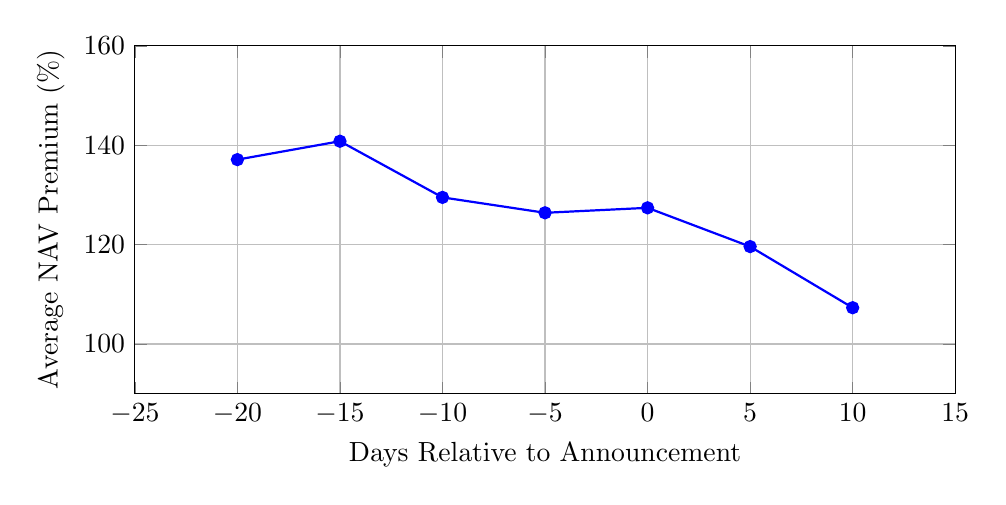
\begin{tikzpicture}
        \begin{axis}[
            width=12cm, height=6cm,
            xlabel={Days Relative to Announcement},
            ylabel={Average NAV Premium (\%)},
            xmin=-25, xmax=15,
            ymin=90, ymax=160,
            grid=major
        ]
        \addplot[thick, blue, mark=*] coordinates {
            (-20, 137.1) (-15, 140.8) (-10, 129.5) (-5, 126.4) (0, 127.4) (5, 119.6) (10, 107.3)
        };
        \end{axis}
    \end{tikzpicture}
    \caption[NAV Premium Around Capital Raise Announcements]{Average NAV premium around capital raise announcements ($N = 23$). Day 0 is the announcement date.}
    \label{fig:event_study}
\end{figure}

\subsection{Scenario Analysis}

Table~\ref{tab:scenarios_results} presents the capital structure under stress scenarios.

\begin{table}[H]
\centering
\caption{Scenario Analysis}
\label{tab:scenarios_results}
\begin{tabular}{@{}lcccc@{}}
\toprule
\textbf{Scenario} & \textbf{BTC Price} & \textbf{NAV} & \textbf{Asset/Debt} & \textbf{Equity Value} \\
\midrule
Base Case & \$95,000 & \$67.8B & 4.25$\times$ & \$51.8B \\
Moderate ($-$30\%) & \$66,500 & \$47.4B & 2.98$\times$ & \$31.5B \\
Severe ($-$50\%) & \$47,500 & \$33.9B & 2.13$\times$ & \$17.9B \\
Prolonged ($-$70\%) & \$28,500 & \$20.3B & 1.28$\times$ & \$4.4B \\
\bottomrule
\end{tabular}
\end{table}

A 50\% BTC drawdown (which has occurred in every historical cycle) compresses equity value from \$51.8 billion to \$17.9 billion, a 65\% decline. The asset/debt ratio falls from 4.25$\times$ to 2.13$\times$, still above the 1.0$\times$ threshold but with less cushion.

The prolonged bear scenario ($-70\%$ BTC) pushes equity to roughly \$4.4 billion (a 92\% decline). At that level, preferred dividends consume a meaningful fraction of remaining equity value, and continued servicing depends on the USD reserve and capital market access.

